
\section{Acceleration techniques}



\subsection{Coarse-to-fine continuation via warm starts}

To reduce the time-to-solution on fine discretizations, we adopt a coarse-to-fine continuation strategy that exploits the warm-start capability of ADMM. 
After solving the SOCP on a coarse mesh, we store (i) the coarse mesh geometry and connectivity, and (ii) the converged ADMM variables from the previous iteration $(x^k,s^k,y^k)$. 
When a refined mesh is generated, these quantities are transferred to initialize the solver on the refined discretization. 
The same strategy applies to both two- and three-dimensional meshes; the only difference is that the simplex element is a triangle in 2D and a tetrahedron in 3D.



\paragraph{Containing element identification with an AABB tree}

A key step in the transfer is to determine, for each point on the refined mesh, the containing element in the coarse mesh. 
We accelerate this search using an axis-aligned bounding box (AABB) tree built over the coarse elements. 
Given a query point's coordinates as input, the AABB tree efficiently identifies candidate coarse elements, after which a point-in-element test is used to determine the containing coarse element. This procedure is illustrated in 2D in Figure~\ref{fig:AABB}; the same approach can be extended straightforwardly to tetrahedral elements in 3D.


\begin{figure}[htbp]
  \centering
  
\includegraphics[width=0.9\textwidth]{figures/Res_To_Date/AABB_scheme.png}
  \caption{How AABB locates the containing element of a given query point}
  \label{fig:AABB}
\end{figure}


\paragraph{Element-level initialization}

For each refined element, we first compute its centroid and identify the corresponding parent element in the coarse mesh using the AABB tree. 
Element-associated quantities, such as the dual variables associated with intra-element equilibrium constraints, are then mapped from the parent coarse element to the refined element.


\paragraph{Stress-point interpolation via barycentric coordinates}

We then initialize the variables at the stress points of each refined element. 
For a given stress point $\mathbf{p}$ located inside a coarse simplex element with vertices $\{\mathbf{v}_j\}_{j=1}^{n_v}$, we compute its barycentric coordinates $\{\lambda_j\}_{j=1}^{n_v}$, where $n_v$ , the number of vertices for an element, $n_v=3$ for a triangle in 2D and $n_v=4$ for a tetrahedron in 3D. 
The warm-start value is then obtained by interpolation:
\begin{equation}
x_0(\mathbf{p}) = \sum_{j=1}^{n_v} \lambda_j \,
x^{\mathrm{coarse}}(\mathbf{v}_j),
\label{eq:interpolation_x}
\end{equation}
with $s_0(\mathbf{p})$ and $y_0(\mathbf{p})$ initialized analogously. 
This formulation provides a dimension-independent transfer rule and allows higher-order discretizations to be warm-started without requiring a prior higher-order solution; in practice, a converged linear-element solution is sufficient.

\subsection{Active cone identification}

ADMM naturally suffers from its linear convergence, and its performance largely depends on the choice of the penalty parameter in the augmented Lagrangian~\cite{SuperADMM}. Following the adaptive penalty updating strategy in~\cite{SuperADMM}, we extend it to SOC constraints by exploiting information from the projection step.

For each SOC block, we consider the slack vector $\boldsymbol{s}_i$. During projection, the block is mapped either onto the cone apex or onto the boundary, that is, when $|| \boldsymbol{r}_i || \le -t_i$  or $ || \boldsymbol{r}_i || > t_i$. We consider the $i$th cone as active whenever either of these conditions holds. After identifying the active cones, we choose to update the diagonal penalty matrix $D(\rho)$ every 20 iterations. This procedure is further illustrated in Figure~\ref{fig:active_cone}

\begin{figure}
\centering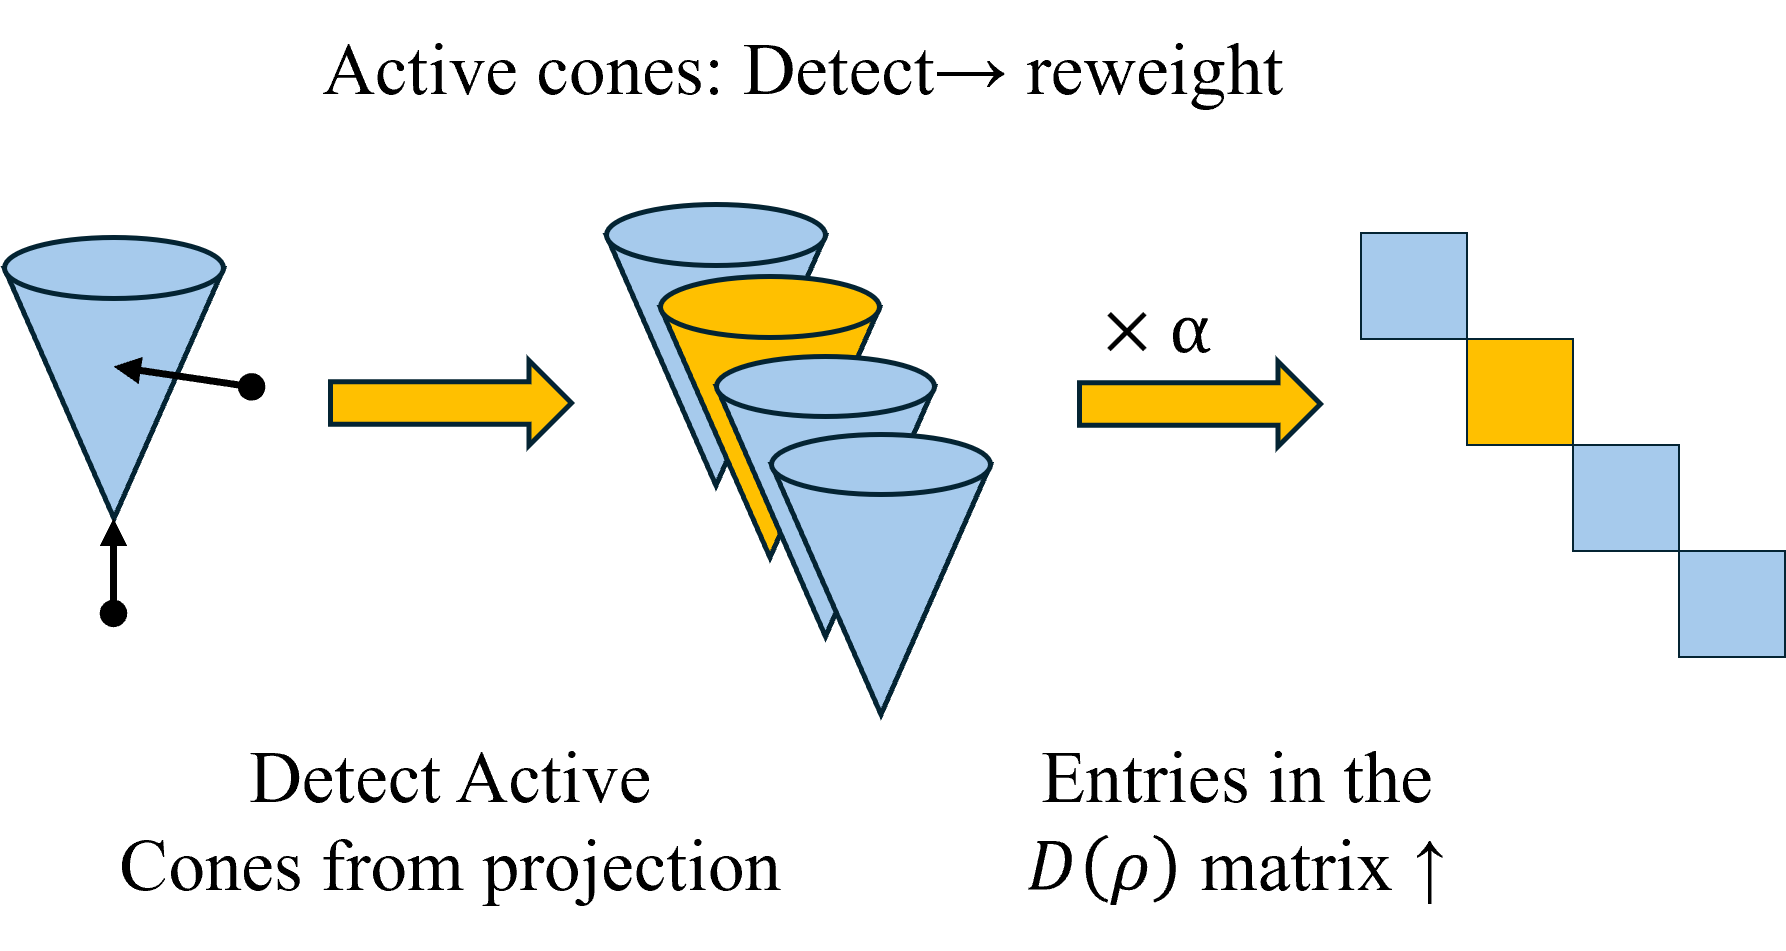
\includegraphics[width=0.70\textwidth]{figures/Res_To_Date/active_cone.png} 
\caption{Active cone identification scheme}
\label{fig:active_cone}
\end{figure}


A fixed bound $B^k$ is imposed to limit the value of the entries of $D(\rho)$ to prevent the system from becoming ill-conditioned. We denote the $j$-th entry of the  diagonal matrix $D(\rho)$ as $D(\rho)_{j,j}^k$, we clamp all entries associated with the SOC blocks to the interval:
\begin{equation}
1/B^k\leq D(\rho)_{j,j}^k\leq B^k
\label{eq:FixedBound}
\end{equation}


Since the penalty is associated with each SOC block, any update to the $D(\rho)$ matrix, must scale all diagonal entries corresponding to the same cone to maintain consistent enforcement. If the cone is active, we multiply all the associated entries by $\alpha$, otherwise do nothing. 
\begin{equation}
D(\rho)^{k+1}_{j,j} =
\begin{cases}
\alpha D(\rho)^{k}_{j,j}, &\text{if } || \boldsymbol{r}_i || \le -t_i$  or $ || \boldsymbol{r}_i || > t_i\\[2pt]
D(\rho)^{(k)}_{j,j}, & \text{otherwise},
\end{cases}
\label{eq:updateDMat}
\end{equation}


Also, at the first 200 iterations, we enforce $\alpha = 2$ when the active set is uncertain at the first 200 iterations. After the stabilization phase, we set $\alpha = 10$ for a more aggressive update. Also, we implement a simple yet effective adaptive adjustment mechanism of the value $\alpha$ near convergence, the heuristic is to reduce $\alpha$ smoothly via a quadratic rule as the iterates approach convergence, avoiding abrupt changes that could destabilize the system or perturb the final solution.

The above updates only happen if the system satisfies the following criteria:
\begin{equation}
r_{\text{dual}} \leq 0.1  \varepsilon_\mathrm{dual}
\label{eq:updateCriteria}
\end{equation} i.e., the dual feasibility condition is already well satisfied, whereas the primal residual remains far from convergence. In practice, with a reasonable initial choice of $\rho$, the dual residual typically decreases to its tolerance earlier than the primal residual.

These simple heuristics prevent the $D(\rho)$ matrix from changing drastically when approaching convergence, while preserving a robust way of updating the variables in a way that the primal and dual residuals are balanced. The idea of balancing these two residuals is inspired by the OSQP solver~\cite{OSQP}, which also adopted an adaptive $\rho$ measure, however the parameter $\rho$ updated uniformly across all constraints, whereas here we adaptively update the penalty only on the active conic blocks.

Notice that the linear constraints are unchanged during the process. Updates to the diagonal weighting matrix $D(\rho)$ modify the system matrix $A^\top D(\rho) A$. Importantly, since $D(\rho)$ only rescales constraint rows, these updates do not change the sparsity pattern of $A^\top D(\rho) A$. We therefore reuse the symbolic factorization and perform only a numerical refactorization of $A^\top D(\rho) A$ whenever $D(\rho)$ is updated, reducing the overhead of re-factorization.




\subsection{Augmented ADMM formulation}

In the GPU-accelerated 3D FELA implementation, we found that even medium-sized problems can exceed the capabilities of a relatively modest GPU (in our case, an NVIDIA RTX A1000). In practice, we observed that in 3D FELA, the condensed matrix becomes increasingly dense as the problem size grows, while the ratio of $\frac{A^\top D(\rho) A.nnz()}{A.nnz()}$ remained close to constant in 2D. This motivated us to solve the augmented linear system rather than the condensed system, with the expectation that the augmented form would lead to fewer non-zero fill-ins during factorization. In practice, we always solve the augmented linear system in 3D.

To improve the conditioning of the linear system, a regularization parameter \(\sigma\) is introduced. Although the augmented system is no longer positive definite, it remains quasi-definite and therefore admits a well-defined \(LDL^\top\) factorization~\cite{COSMO}:

\begin{equation}
\begin{bmatrix}
\sigma I & A^{T} \\
A & -D(\rho)^{-1}
\end{bmatrix}
\begin{bmatrix}
x^{k+1} \\
\upsilon
\end{bmatrix}
=
\begin{bmatrix}
-c + \sigma x^{k} \\
b - s - D(\rho)^{-1} y
\end{bmatrix}
\label{eq:AUG}
\end{equation}

 

\subsection{Alternative ellipsoidal projection scheme}

Solver performance may also be improved by adopting an alternative projection strategy. In MOSEK and in our ADMM implementation, the projection step is introduced by adding an additional set of variables \(s\) and enforcing
$Ax + s = b$,
where, for each conic constraint, \(A\) is the affine transformation matrix defined in \eqref{eq:2DSOC}. When \(\alpha = 0\), the Drucker--Prager criterion reduces to the von Mises criterion, and the corresponding SOC projection becomes equivalent to a projection onto an ellipsoid.

This ellipsoidal projection scheme was implemented only in the 3D programme. After splitting and enforcing \(x = s\), the projection step at each stress point \(i\) amounts to projecting the associated slack vector
\[
s_i^{\mathrm{trial}} = (s_{1,i}, s_{2,i}, \dots, s_{6,i})^\top
\]
onto the ellipsoid
\[
\mathcal{E} = \{\, s \in \mathbb{R}^6 \mid s^\top P s \leq 1 \,\}.
\]

The projection problem can therefore be written as
\begin{equation}
\begin{array}{ll}
\textbf{minimize}   & \dfrac{1}{2}\|s - s_i^{\mathrm{trial}}\|^2 \\[4pt]
\textbf{subject to} & s^\top P s \leq 1,
\end{array}
\label{eq:ELP}
\end{equation}
where \(s_i^{\mathrm{trial}}\) denotes the current slack vector before projection.

For stress points lying outside the ellipsoid, the inequality constraint is active at the solution, and the KKT conditions are
\begin{equation}
\begin{array}{ll}
1) & s - s_i^{\mathrm{trial}} + 2\lambda P s = 0, \\[4pt]
2) & s^\top P s = 1, \\[4pt]
3) & \lambda \geq 0.
\end{array}
\label{eq:KKT_ELP}
\end{equation}
Let
\[
\mu = 2\lambda \geq 0.
\]
Then we obtain
\begin{equation}
(I + \mu P)s = s_i^{\mathrm{trial}},
\end{equation}
and hence
\begin{equation}
s(\mu) = (I + \mu P)^{-1} s_i^{\mathrm{trial}}.
\end{equation}

We now give the formulation of the P matrix as:
\begin{equation}
P = \frac{1}{k^2}
\begin{bmatrix}
\frac{1}{3} & -\frac{1}{6} &  -\frac{1}{6} & 0 & 0 & 0 \\
-\frac{1}{6} & \frac{1}{3} &  -\frac{1}{6} & 0 & 0 & 0 \\
-\frac{1}{6} & -\frac{1}{6} & \frac{1}{3} &  0 & 0 & 0 \\
0 & 0 & 0 & 1 & 0 & 0 \\
0 & 0 & 0 & 0 & 1 & 0 \\
0 & 0 & 0 & 0 & 0 & 1 
\end{bmatrix}
\end{equation}
Substituting \(s(\mu)\) into the active constraint yields the scalar root-finding problem
\begin{equation}
\phi(\mu) = s(\mu)^\top P s(\mu) - 1 = 0,
\end{equation}
which can be solved efficiently by Newton's method:
\begin{equation}
\mu_{j+1} = \mu_j - \frac{\phi(\mu_j)}{\phi'(\mu_j)}.
\label{eq:Newt}
\end{equation}

In practice, although a large number of stress points must be projected, the high-level parallelisation provided by a customised CUDA kernel reduces the cost of this step to only about \(3\%\) of the total solution time.

\subsection{Implementation of the solver on CUDA}

Profiling of the code on CPU showed that apart from the obvious bottleneck of the solve operation that took place in every iteration, the various sparse matrix manipulations, if not handled efficiently, may also significantly degrade overall solver performance. To address this, the implementation makes intensive use of GPU acceleration, and the following improvements were made:

\paragraph{cuDSS for solving the linear system}



In the condensed formulation, the KKT system is symmetric positive-definite. As a result, cuDSS internally uses a Cholesky factorization path, which is faster and more memory-efficient than the general-purpose $LDL^\top$ decomposition. This choice leads to significant runtime improvements in the solve phase of each ADMM iteration in 2D FELA, however, in 3D, when memory usage of a condensed formulation exceeds the capacity of the GPU, the augmented formulation, even though it used a sparse $LDL^\top$ decomposition, was faster in time per-iteration.

\paragraph{cuBLAS and cuSPARSE for efficient construction of vectors}

cuBLAS is a CUDA implementation of BLAS, which enables convenient access to GPU-accelerated BLAS operations. cuSPARSE is a CUDA library that contains many commonly used matrix manipulation subroutines. 

\paragraph{CUDA kernel functions for customized variable updates}

CUDA kernel functions are special C functions executed on the GPU in a highly parallelised fashion~\cite{GPU_ADMM}. Each thread runs the same instructions on different data, making them inherently suitable for SIMD-style computations. While many standard linear algebra operations are efficiently handled by highly optimized libraries such as cuBLAS and cuSPARSE, several complex or non-standard operations required in our solver are not directly supported. 

For example, the non-uniform scaling of the variables and matrices, and simultaneous projection onto $N_{SOC}$ second-order cones, and parallel updates of intermediate vectors fall outside of the scope of existing CUDA libraries. 

\paragraph{All operations completed on GPU}

Though the construction of the KKT matrix and warm-starting is completed outside of the GPU, all the subsequent ADMM iterations are completed on the GPU, only passing the primal and dual residual and the current objective back to the CPU. This design significantly eliminated the overhead introduced by the frequent GPU-CPU data transfers.
